\section{Results}\label{sec:results}

\subsection{OLS Benchmark}

Column 1 of Table~\ref{tab:main_qr} reports the survey-weighted OLS estimates. The SIS coefficient is small and statistically insignificant ($\hat{\beta} = 0.0032$, $\text{SE} = 0.0028$), indicating that, on average, SIS membership is not associated with a meaningfully different OOP share relative to being uninsured, conditional on quintile, demographics, and region. The EsSalud coefficient is large (0.2359) but imprecise ($\text{SE} = 0.2039$), reflecting the small EsSalud cell size ($N = 648$) discussed in Section~\ref{sec:data}; we caution against interpreting this estimate.

Consumption quintile dummies display a monotonically increasing pattern: relative to Q1, households in Q2 through Q5 have progressively higher OOP shares, with the Q5 coefficient at 2.23 percentage points ($p < 0.01$). This gradient is expected but should be interpreted with the caveat that quintile assignment includes health spending in the denominator (Section~\ref{sec:data}), which mechanically inflates the quintile--OOP share correlation.

The SIS--quintile interactions are uniformly negative but individually insignificant in OLS, with the SIS$\times$Q5 interaction at $-0.0102$ ($\text{SE} = 0.0065$). The OLS $R^2$ is 0.0201, reflecting the high residual variance characteristic of health expenditure regressions.

\subsection{Quantile Regression: Main Results}

Columns 2--6 of Table~\ref{tab:main_qr} report the conditional quantile regression estimates at $\tau = \{0.10, 0.25, 0.50, 0.75, 0.90\}$.

\begin{table}[htbp]
\centering
\caption{Quantile Regression: Insurance Associations with OOP Share}
\label{tab:main_qr}
\scriptsize
\begin{tabular}{lcccccc}
\toprule
& OLS & $\tau=0.1$ & $\tau=0.25$ & $\tau=0.5$ & $\tau=0.75$ & $\tau=0.9$ \\
\midrule
  SIS & 0.0032 & 0.0000 & 0.0000 & -0.0000 & 0.0013 & 0.0047 \\
  & (0.0028) & (0.0000) & (0.0000) & (0.0001) & (0.0010) & (0.0051) \\
  EsSalud & 0.2359 & 0.0000 & 0.0000 & 0.0005 & 0.0002 & 0.9183** \\
  & (0.2039) & (0.0000) & (0.0003) & (0.0006) & (0.3127) & (0.4551) \\
  Q2 & 0.0073*** & 0.0000*** & 0.0000*** & 0.0006*** & 0.0052*** & 0.0144*** \\
  & (0.0017) & (0.0000) & (0.0000) & (0.0001) & (0.0007) & (0.0022) \\
  Q3 & 0.0118*** & 0.0000*** & 0.0000*** & 0.0022*** & 0.0085*** & 0.0263*** \\
  & (0.0021) & (0.0000) & (0.0000) & (0.0003) & (0.0008) & (0.0026) \\
  Q4 & 0.0155*** & 0.0000*** & 0.0000 & 0.0046*** & 0.0128*** & 0.0309*** \\
  & (0.0032) & (0.0000) & (0.0000) & (0.0004) & (0.0011) & (0.0037) \\
  Q5 & 0.0223*** & 0.0000*** & 0.0010*** & 0.0057*** & 0.0188*** & 0.0516*** \\
  & (0.0054) & (0.0000) & (0.0003) & (0.0006) & (0.0020) & (0.0048) \\
  SIS $\times$ Q2 & -0.0057 & -0.0000 & -0.0000 & -0.0003 & -0.0032** & -0.0069 \\
  & (0.0049) & (0.0000) & (0.0000) & (0.0002) & (0.0016) & (0.0062) \\
  SIS $\times$ Q3 & -0.0057 & -0.0000*** & -0.0000*** & -0.0010*** & -0.0036** & -0.0147** \\
  & (0.0043) & (0.0000) & (0.0000) & (0.0003) & (0.0015) & (0.0059) \\
  SIS $\times$ Q4 & -0.0075 & -0.0000*** & -0.0000 & -0.0022*** & -0.0065*** & -0.0107* \\
  & (0.0050) & (0.0000) & (0.0000) & (0.0005) & (0.0015) & (0.0063) \\
  SIS $\times$ Q5 & -0.0102 & -0.0000*** & -0.0010*** & -0.0017** & -0.0057** & -0.0194*** \\
  & (0.0065) & (0.0000) & (0.0003) & (0.0007) & (0.0026) & (0.0073) \\
  EsSalud $\times$ Q2 & -0.2480 & -0.0000 & -0.0000 & -0.0008 & -0.0076 & -0.8944* \\
  & (0.2041) & (0.0000) & (0.0003) & (0.0014) & (0.3118) & (0.4580) \\
  EsSalud $\times$ Q3 & -0.2606 & -0.0000*** & -0.0000 & -0.0036*** & -0.0039 & -0.9364** \\
  & (0.2039) & (0.0000) & (0.0003) & (0.0014) & (0.3126) & (0.4557) \\
  EsSalud $\times$ Q4 & -0.2547 & -0.0000*** & -0.0000 & -0.0046*** & -0.0128 & -0.9299** \\
  & (0.2040) & (0.0000) & (0.0003) & (0.0007) & (0.3125) & (0.4544) \\
  EsSalud $\times$ Q5 & -0.2390 & -0.0000*** & -0.0010*** & -0.0047*** & -0.0081 & -0.9467** \\
  & (0.2041) & (0.0000) & (0.0004) & (0.0010) & (0.3127) & (0.4546) \\
\midrule
  N & 33,691 & 33,691 & 33,691 & 33,691 & 33,691 & 33,691 \\
  R$^2$/Pseudo-R$^2$ & 0.0201 & -0.0000 & 0.0021 & 0.0252 & 0.0351 & 0.0426 \\
\bottomrule
\end{tabular}
\begin{minipage}{\textwidth}\footnotesize
\textit{Notes:} Coefficients represent changes in the conditional $\tau$-quantile of OOP
health expenditure share, not average marginal effects. Causal interpretation is not warranted
given non-random insurance assignment. OLS is survey-weighted (FACTOR07) with cluster-robust SEs.
QR uses cluster-bootstrapped SEs (200 reps, PSU-level). Q1 and Uninsured are omitted.
*** p$<$0.01, ** p$<$0.05, * p$<$0.10.
\end{minipage}
\end{table}

\paragraph{Low quantiles ($\tau = 0.10, 0.25$): uninformative due to zero mass.} At $\tau = 0.10$, all coefficients are at or near zero with negligible standard errors, confirming the degeneracy of the conditional quantile function at quantiles below the 44.1\% zero-OOP mass. At $\tau = 0.25$, coefficients begin to differentiate---Q5 shows a significant positive association (0.0010, $p < 0.01$), and the SIS$\times$Q5 interaction offsets it ($-0.0010$, $p < 0.01$)---but these effects are economically trivial, representing movements between zero and near-zero OOP shares. \textbf{We do not interpret these estimates substantively}; they are reported for completeness and illustrate why standard CQR is uninformative at lower quantiles with large zero mass \citep{MachadoSilva2005}.

\paragraph{Median ($\tau = 0.50$).} At the median, the quintile gradient is established: Q2 through Q5 are associated with progressively higher conditional OOP shares (Q5: 0.57 percentage points, $p < 0.01$). The SIS base coefficient remains insignificant ($-0.0000$, $p = 0.89$). The SIS--quintile interactions are negative and significant for Q3 ($-0.10$ pp, $p < 0.01$), Q4 ($-0.22$ pp, $p < 0.01$), and Q5 ($-0.17$ pp, $p < 0.05$), indicating that at the median, SIS membership is associated with reduced OOP share for households in the upper half of the consumption distribution. We note that these magnitudes are small in absolute terms and that significance conclusions are subject to the multiple testing caveat discussed in Section~\ref{sec:strategy}.

\paragraph{Upper quantiles ($\tau = 0.75, 0.90$).} The quintile gradient steepens substantially. At $\tau = 0.75$, Q5 households have a conditional OOP share 1.88 percentage points higher than Q1 ($p < 0.01$). At $\tau = 0.90$, this gap widens to 5.16 percentage points ($p < 0.01$). The SIS--quintile interactions are correspondingly larger: at $\tau = 0.90$, SIS$\times$Q3 reduces OOP share by 1.47 percentage points ($p < 0.05$), and SIS$\times$Q5 by 1.94 percentage points ($p < 0.01$). At $\tau = 0.90$, SIS membership is associated with a reduction in OOP share of roughly one-third of the quintile gradient for Q5 households.

These upper-tail findings should be interpreted cautiously for three reasons. First, the 200-replication bootstrap may produce noisy standard errors at $\tau = 0.90$, where effective cell sizes are small. Second, the monotonic pattern---where SIS protection increases with quintile rank---does not support a middle-income squeeze but rather suggests a regressive protection gradient, as we discuss below. Third, SIS enrollment at Q4--Q5 reflects targeting leakage \citep{Cortez2008}, and the interaction coefficients conflate insurance protection with the composition of the (mis)targeted population.

\subsection{Total Insurance Association by Quintile}

Table~\ref{tab:total_effect} reports the total insurance association---the sum of the base coefficient and the relevant interaction term---for each insurance--quintile--quantile cell.

\begin{table}[htbp]
\centering
\caption{Total Insurance Association with OOP Share by Quintile}
\label{tab:total_effect}
\small
\begin{tabular}{llccccc}
\toprule
Insurance & Quintile & $\tau=0.1$ & $\tau=0.25$ & $\tau=0.5$ & $\tau=0.75$ & $\tau=0.9$ \\
\midrule
  SIS & Q1 & +0.0000 & +0.0000 & -0.0000 & +0.0013 & +0.0047 \\
   & Q2 & -0.0000 & -0.0000 & -0.0003 & -0.0019 & -0.0023 \\
   & Q3 & -0.0000*** & -0.0000*** & -0.0010*** & -0.0023 & -0.0100 \\
   & Q4 & -0.0000*** & -0.0000 & -0.0022*** & -0.0052*** & -0.0060 \\
   & Q5 & -0.0000*** & -0.0010*** & -0.0017** & -0.0044 & -0.0147* \\
\midrule
  EsSalud & Q1 & +0.0000 & +0.0000 & +0.0005 & +0.0002 & +0.9183** \\
   & Q2 & -0.0000 & -0.0000 & -0.0003 & -0.0074 & +0.0239 \\
   & Q3 & -0.0000* & -0.0000 & -0.0031** & -0.0036 & -0.0181 \\
   & Q4 & -0.0000** & -0.0000 & -0.0041*** & -0.0126 & -0.0116 \\
   & Q5 & -0.0000* & -0.0010** & -0.0041*** & -0.0079 & -0.0283 \\
\bottomrule
\end{tabular}
\begin{minipage}{\textwidth}\footnotesize
\textit{Notes:} Total association = base coefficient + interaction.
Cluster-bootstrapped SEs (200 reps). *** p$<$0.01, ** p$<$0.05, * p$<$0.10.
\end{minipage}
\end{table}

For SIS, the total association at Q1 is statistically insignificant across all quantiles, confirming that SIS membership does not differentiate OOP burden among the poorest households. At higher quintiles, negative associations emerge and grow with both the quintile and the quantile: at Q5, the total SIS association is $-0.0017$ at $\tau = 0.50$ ($p < 0.05$) and $-0.0147$ at $\tau = 0.90$ ($p < 0.10$).

This pattern forms a \textbf{monotonic protection gradient}: the magnitude of the SIS association increases steadily from Q1 to Q5 and from $\tau = 0.50$ to $\tau = 0.90$. This is inconsistent with the middle-income squeeze hypothesis, which predicts that Q2--Q4 households face disproportionate OOP burden relative to \textit{both} Q1 and Q5. Instead, the evidence is more consistent with regressive financial protection---insurance protection increases with income, conditional on enrollment---a coverage incidence finding rather than a squeeze.

EsSalud results are reported in Table~\ref{tab:total_effect} for completeness but are excluded from substantive interpretation. The EsSalud sample ($N = 648$) is implausibly small, likely reflecting the household-head-based insurance assignment that misclassifies households with non-head EsSalud members as uninsured. This misclassification contaminates the uninsured reference group and may bias the SIS interaction estimates. The anomalous $\tau = 0.90$ coefficient for EsSalud Q1 (0.9183) is driven by a cell with fewer than 30 observations and is not meaningful. Correcting the insurance variable construction---using any-member EsSalud coverage rather than head-only---is a prerequisite for credible EsSalud analysis and would also improve the SIS estimates by decontaminating the reference group.

\subsection{Distributional Evidence}

Figures~\ref{fig:kde} through \ref{fig:che} provide visual evidence.

\begin{figure}[htbp]
    \centering
    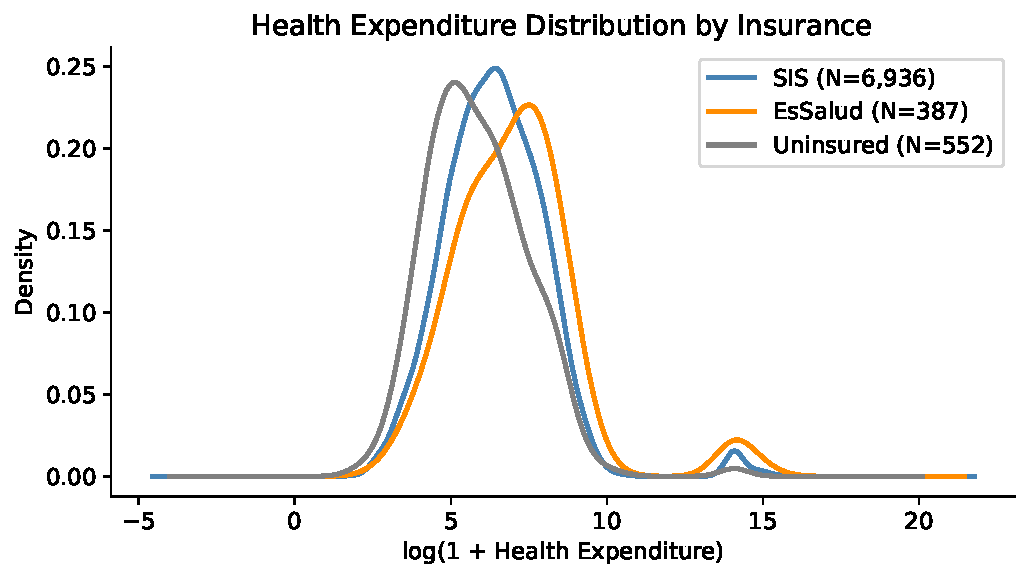
\includegraphics[width=0.85\textwidth]{figures/fig1_kde_expenditure.pdf}
    \caption{Kernel density of OOP health expenditure share by insurance group (survey-weighted). The vertical dashed lines indicate the 10\% and 25\% CHE thresholds.}
    \label{fig:kde}
\end{figure}

Figure~\ref{fig:kde} displays the weighted kernel density of OOP share by insurance group. All three distributions are concentrated near zero, with long right tails. The uninsured distribution has the thinnest right tail, consistent with care avoidance rather than financial protection.

\begin{figure}[htbp]
    \centering
    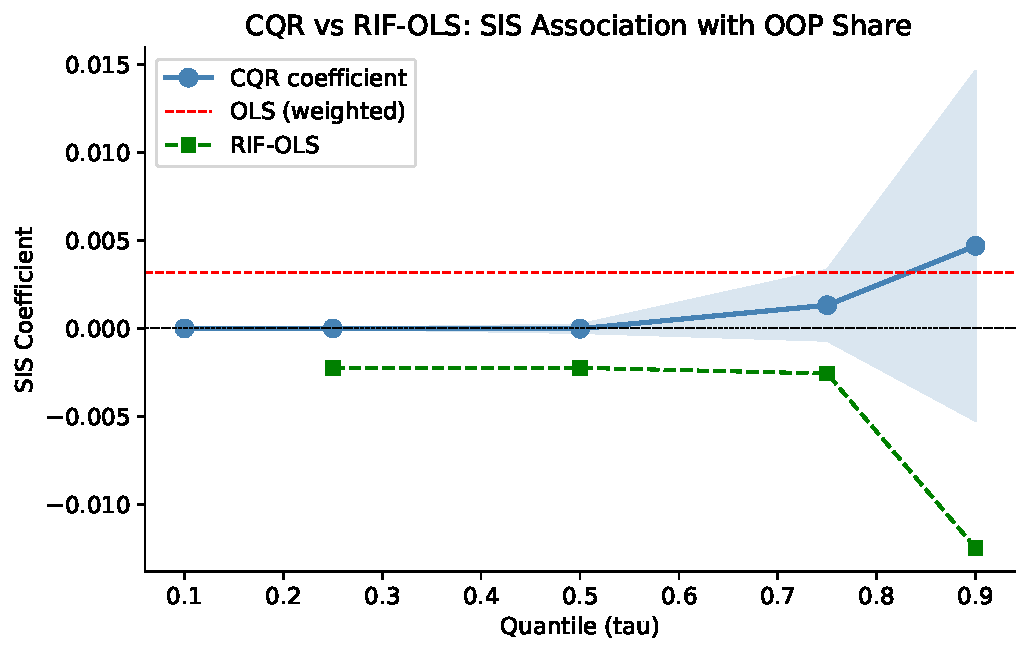
\includegraphics[width=0.85\textwidth]{figures/fig2_qte_plot.pdf}
    \caption{Quantile treatment effect profile: SIS coefficient across quantiles with 95\% confidence bands. Estimates at $\tau < 0.50$ are uninformative due to zero-mass degeneracy.}
    \label{fig:qte}
\end{figure}

\begin{figure}[htbp]
    \centering
    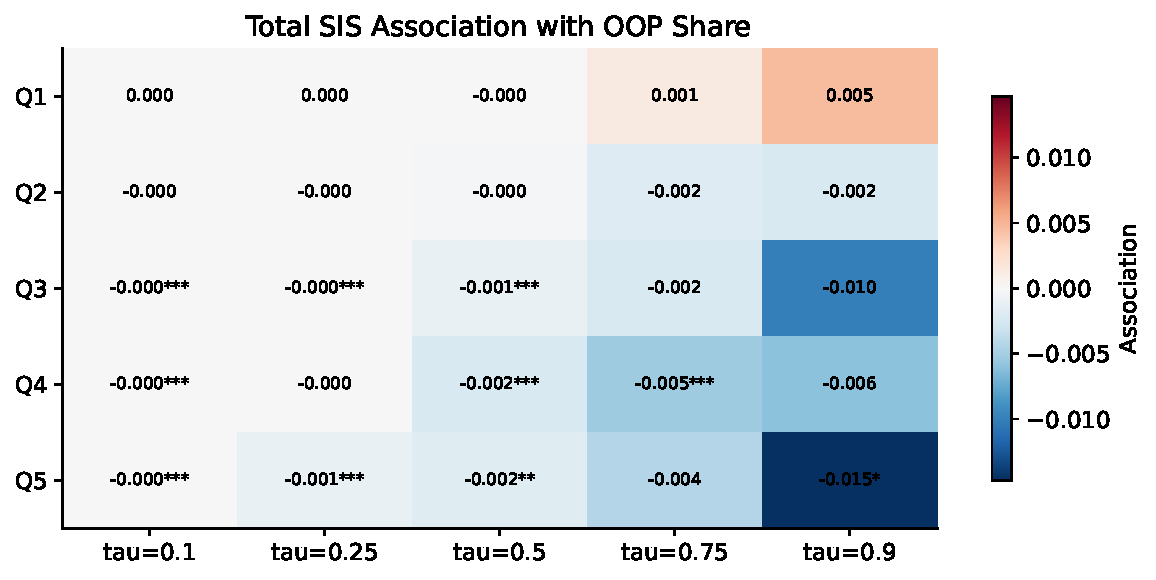
\includegraphics[width=0.85\textwidth]{figures/fig3_heatmap_total_effect.pdf}
    \caption{Heatmap of total SIS association with OOP share by consumption quintile and quantile. Darker shading indicates larger negative associations (greater financial protection).}
    \label{fig:heatmap}
\end{figure}

Figure~\ref{fig:heatmap} presents the total SIS association as a heatmap. The gradient from white (Q1, lower quantiles) to dark (Q5, upper quantiles) visualizes the monotonic protection gradient: SIS is differentially associated with OOP burden at higher points of both the income and spending distributions.

\begin{figure}[htbp]
    \centering
    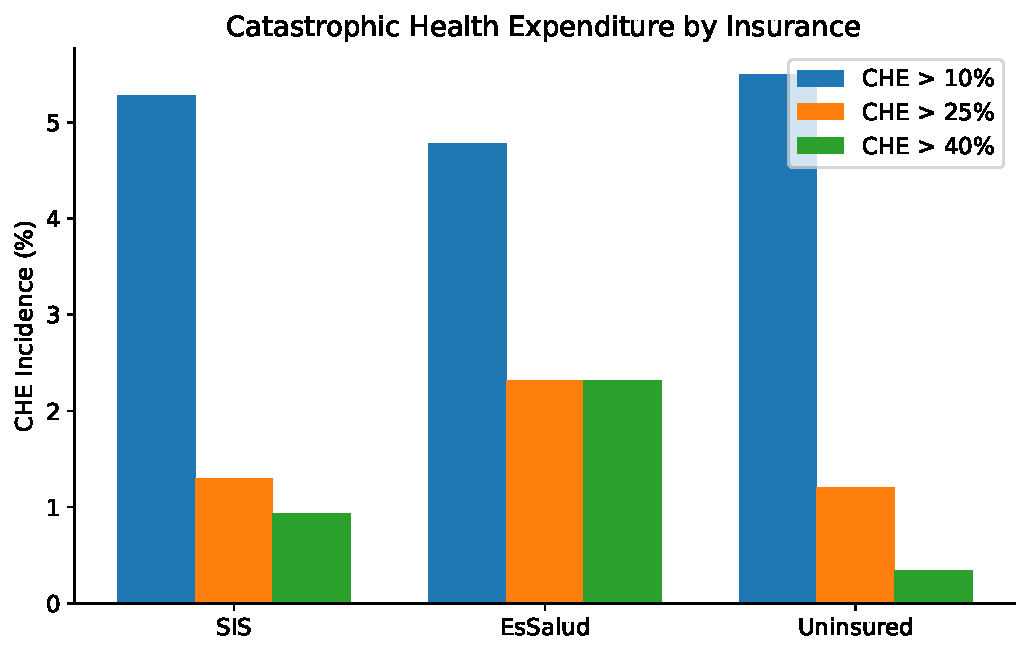
\includegraphics[width=0.85\textwidth]{figures/fig4_che_by_insurance.pdf}
    \caption{CHE incidence by insurance group and consumption quintile at the 10\% threshold.}
    \label{fig:che}
\end{figure}
